\section{Deep Learning for Image Segmentation} \label{sec:deep-learning-and-neural-networks}
In the following section, a short introduction to deep learning and especially neural networks and (vision) transformers will be given in order to understand how \gls{stego} can be adapted for scientific data.
In deep learning, multilayer neural networks (or deep neural networks) are used to solve a wide variety of tasks, ranging from classification and clustering to discovering relationships between features of examples (i.e.\ regression), or dimensionality reduction~\autocite{Sarker2021}.
Since image segmentation is just a multilevel pixel classification, it can be easily cast into a deep learning problem, and some algorithms were even found to exceed human performance in quality and time~\autocite{Alzubaidi2021}.

\subsection{Algorithm Categories}
Traditionally, algorithms are classified into three categories:
supervised algorithms, trained on data where ground truth is available, unsupervised algorithms, where ground truth is not available, and reinforcement learning, which is tailored to solve problems where the decision-making process is sequential.
In the last years, also semi-super\-vised algorithms were differentiated, which combine supervised and unsupervised learning, which try to get the best of both worlds.
They are used on data where ground truth is available only on some samples.~\autocite{Burkov2019}

Image segmentation can be done with all three of them, but to date the best results are reached with supervised algorithms like convolutional neural networks or U-Nets~\autocite[e.g.][]{Isensee2019}.
%, though Unsupervised and Semi-supervised Learning are also found increasingly successful~\autocite[e.g.]{VanGansbeke2021}.\footnote{Reinforcement Learning on the other hand, is better tailored to solve problems where the decision-making process is sequential (for example when playing video games or in navigation).} %Reinforcement can be used for segmentation, but that is not classical application https://arxiv.org/abs/2002.06583
%disadvantages of Supervised algorithms and transition
However, these supervised networks do come with a major disadvantage: their need for labelled data.
As it is in the nature of labels to be assigned manually (and for scientific images often even by domain experts which are rare), data preparation takes a lot of time, which is usually not feasible.

%unsupervised learning
This is why today, there are increasing efforts to leverage unsupervised learning techniques, which find an arbitrary structure within the input without getting feedback from ground truth labels~\autocite{Burkov2019}.
Only recently, unsupervised Deep Learning algorithms for image segmentation were presented for 2D pictures, either based on a convolutional neural network~\autocite{VanGansbeke2021} or a vision transformer~\autocite{Caron2021}.
But to date, no unsupervised algorithm is available for scientific imaging data.


\subsection{Deep Neural Networks}
All deep learning algorithms rely on multilayer neural networks.
Originally, artificial neural networks were based on the idea to model biological neurons and especially the connection of neurons (since the connections carry the real information), to enable computers to learn in the same way humans do~\autocite{Ertel2017}.
Today, they are used for a wide variety of tasks, ranging from classification, and clustering, over regression, to dimensionality reduction~\autocite{Sarker2021}.

% how multilayer networks work (roughly)
Multilayer networks are created by using the output of a set of neurons (the layer) as input for the next layer of neurons~\autocite[Chapter~4.2]{Skansi2018}.
Usually, there are no interlayer connections and all neurons of the previous layer are connected to all neurons of the next layer, but this may change with the network architecture~\autocite[Chapter~1.2.2]{Aggarwal2018}.
Each neuron is appointed a set of weights which is multiplied with the input(s) to calculate the output of that neuron~\autocite[Chapter~4.2]{Skansi2018}.
This is done throughout all layers (forward pass).
On the backward pass, the learning is done by purposefully adjusting the weights, so the output of the network will be closer to the desired output~\autocite{Ruder2017}.
In supervised networks, this is done by comparing the output with the label of the training example by means of a loss function~\autocite{Aggarwal2018, Ruder2017}.
In unsupervised networks, the loss function utilises other indicators, as explained exemplarily in~\autoref{sec:stego} for a transformer.
For more details on neural networks, backpropagation and loss functions, see~\autocite[e.g.][]{Pouliakis2016, Sharma2020, Ruder2017}.


\subsection{Model Performance Assessment} \label{subsec:model-performance-assessment}
Once training of a network is finished, and all weights are optimised, the network represents a model, which can be used to predict results for unknown input.
To assess model performance, predictions on a data set not part of the training set are compared to their ground truth~\autocite{Aggarwal2018}.

For classification tasks, the most frequently used assessment metrics rely on the confusion matrix~\autocite{Reinke2022}.
This matrix has two axis, comprising the predicted and actual labels (ground truth), as seen in \autoref{tab:confusion-matrix}.
In a binary classification task, four cardinalities are defined, but it can be easily extended for multilevel classifications by adding a row and column for each label~\autocite{Reinke2022}.
Cardinalities are:
\begin{itemize}
    \item true positives (TP): examples that are correctly predicted to belong to a specific label
    \item false positives (FP): examples that are incorrectly predicted to belong to a specific label
    \item true negatives (TN): examples that are correctly predicted as not belonging to a specific label
    \item false negatives (FN): examples that are incorrectly predicted to not belong to a specific label
\end{itemize}
\vspace{12pt}

\begin{table}[!htb]
    \centering
    \caption[Confusion Matrix for Binary Classification]{Confusion matrix for a binary classification task with the labels \emph{yes} and \emph{no}. It characterises the capabilities of a model by comparing the numbers of actual and predicted examples for each label. The sum within a row gives the number of actual examples with that label, the sum of a column the number of actually predicted examples of that label. The four cardinalities of the table (true positive, false positive, true negative, false negative) are used to calculate metrics that indicate the model performance.}
    \label{tab:confusion-matrix}
    \makegapedcells
    \begin{tabular}{cc|c|c}
        \multicolumn{2}{c|}{}  &   \multicolumn{2}{c}{\textbf{Predicted}}  \\
        &             &      yes       &      no         \\
        \cline{1-4}
        \multirow{2}{*}{\rotatebox[origin=c]{90}{\textbf{Actual}}}
        & yes         & \makecell{true positive \\ (TP)}  &  \makecell{false negative \\ (FN)} \\
        \cline{2-4}
        & no          &  \makecell{false positive \\ (FP)} &  \makecell{true negative \\ (TN)}   \\

    \end{tabular}
\end{table}

%semantic image segmentation assessment score:
The values of the confusion matrix can be used to calculate different metrics, for example the accuracy, but also the \gls{dsc} and the \gls{iou}, which are two of the most commonly used metrics in computer vision and medical image segmentation tasks~\autocite{Reinke2022}.

% Accuracy
In image segmentation, the accuracy represents the proportion of correctly identified pixels.
It is calculated as follows:
\begin{equation}
    Accuracy = \frac{TP + TN}{TP + TN + FP + FN}
    \label{eq:accuracy}
\end{equation}
%DSC
The \gls{dsc} (or F1-score) indicates the overall overlap between the predicted and the actual labels of all pixels (or voxels) as value from 0 (no overlap) to 1 (full overlap)~\autocite{Reinke2022}.
For a single label it is defined as:
\begin{equation}
    DSC = \frac{2TP}{2TP + FP + FN}
    \label{eq:dsc}
\end{equation}
%IoU
The \gls{iou} (or Jaquard-index) is defined as the ratio of area of overlap and area of union, hence the name~\autocite{Reinke2022}:
\begin{equation}
    IoU = \frac{TP}{TP + FP + FN} \text{ or } IoU_{A,B} = \frac{|A \cap B|}{|A \cup B|}
    \label{eq:IoU}
\end{equation}
\gls{iou} and \gls{dsc} are related, as the \gls{dsc} of two sets $A$ and $B$ can also be expressed via the \gls{iou} of these sets~\autocite{Reinke2022}:
\begin{equation}
    DSC_{A,B} = \frac{2IoU_{A,B}}{1 + IoU_{A,B}}
    \label{eq:dsc-IoU}
\end{equation}
When evaluating these metrics, it has to be taken into account, however, that it is just an average and it may be especially misleading when small areas are compared, where a difference of one pixel has a high impact~\autocite{Reinke2022}.
Moreover, it has to be kept in mind that even domain experts often disagree on the exact boundaries of objects in an image~\autocite{Webb2021}.
So when evaluating a model, it is imperative to not rely solely on the metrics, but also have a look on the predictions made.
% limitations of metrics
%When selecting a metric to evaluate a model, the different advantages and limitations must be considered with respect to the task at hand, as explained by~\autocite{Reinke2022}.

% cross validation
Other ways to improve model performance are resampling methods.
In the most basic set-up, available data will be split into train and test set.
The model will be trained on the training set and validation metrics will be calculated on the test set to estimate the model performance (the model's generalisation capacities).
This leaves out a considerable amount of data from the training, and might bias the resulting model.
To mitigate this, often resampling methods are used, where multiple models are trained on different train test splits.
The analysis of these models estimates the performance of the final model (trained on the full data set).
Usually, in machine learning, the so-called k-fold cross validation is done, where the data is split into $k$ sets (or folds) and every fold is used as validation set exactly once.
In practice, $k$ is often set to 5 or 10, depending on the amount of data available.~\autocite[Chapter 5]{James2013}

A special case of cross-validation is leave-one-out cross-validation, where the data set is split into $n$ folds ($n$ indicating the number of samples in the data set).
So, $n$ models are trained, and during each training exactly one sample is used as validation set~\autocite[Chapter 5]{James2013}.
Especially with smaller data sets, a leave-one-out tactic is often recommended, since the algorithm is trained on a more representative training set, thus reducing the bias of the model~\autocite[Chapter 5]{James2013}. %https://codesachin.wordpress.com/2015/08/30/cross-validation-and-the-bias-variance-tradeoff-for-dummies/
However, using only one sample as validation set might lead to a higher variance during evaluations, since inhomogeneities and outliers in the data will have more influence when used alone for validation~\autocite[Chapter 5]{James2013}.
On the other hand, \citeauthor{Bengio2004} found that high correlation of training sets may also lead to a higher variance in leave-one-out cross-validation~\autocite{Bengio2004}. %https://stats.stackexchange.com/questions/61783/bias-and-variance-in-leave-one-out-vs-k-fold-cross-validation
So performance on leave-one-out cross-validation might vary highly between data sets.

\subsection{Transformers}
\label{subsec:transformer}
% http://nlp.seas.harvard.edu/2018/04/01/attention.html#position-wise-feed-forward-networks
% Transformer - Overview
Originally, transformers were developed for (supervised) language processing tasks.
They generally accept sequential input data (e.g.~words in a sentence), while allowing parallel processing.
This sets them apart from the former state-of-the-art in natural language processing (e.g.~recurrent or convolutional neural networks).
In contrast to most other networks, transformers are solely based on an attention mechanism, which can easily be parallelised, and require less computational power, which means they often reach better results with less resources.
Like all encoder-decoders, transformers map an input token\footnote{In this context, a token usually is a word.} to an output token via an intermediate representation of inputs, which should encode all relevant features.~\autocite{Vaswani2017}

% Transformers for images
Due to their good performance, transformers were soon adapted to be applied to image classification, and are today also successfully used as vision transformers for image segmentation tasks~\autocite{Han2023}.
In contrast to most state-of-the-art image segmentation methods, vision transformers have the potential to be trained fully unsupervised~\autocite{Hamilton2022}, making them highly relevant for scientific application, where often no labeled data is available.
However, vision transformers were found to require more data in comparison, as discussed in~\autocite{Coccomini2021}.

\subsubsection{Model Structure}
% Transformer - Model Structure
% https://www.wikiwand.com/en/Transformer_(machine_learning_model)#Architecture
As seen in \autoref{fig:transformer}, transformers implement an encoder-decoder model structure without using convolutions or recurrence, which is instead replaced with multi-head attention and point-wise feedforward networks~\autocite{Vaswani2017}.
\begin{figure}[p]
    \centering
    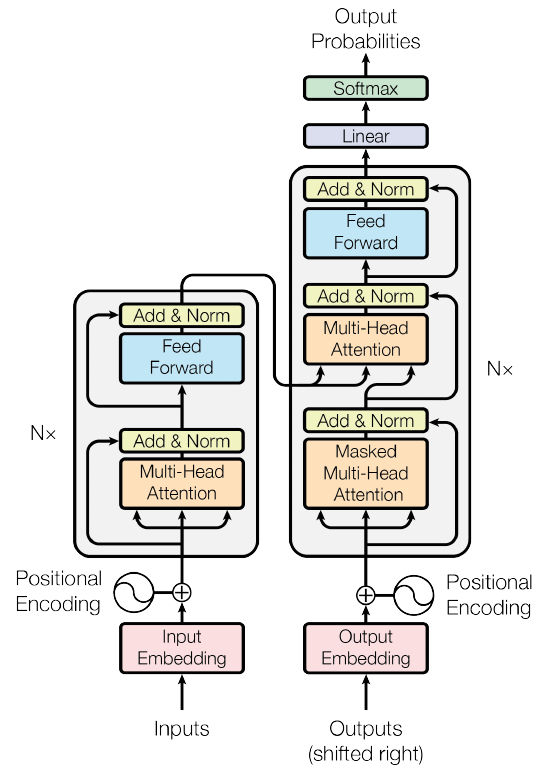
\includegraphics[width=0.75\textwidth]{pictures/transformer}\\
    \caption[Transformer Model Structure]{Transformer model structure. The transformer consists of an encoder (left side) and a decoder (right side). The encoder comprises a multi-head self-attention sublayer and a fully connected feedforward sublayer. Each sublayer has residual connections to the respective input, which is added to the output. The sum is then normalised and passed on to the next sublayer.\\The decoder is structured similarly, but has an additional intermediate layer, where cross-attention with the encoder output is calculated. Also the self-attention sublayer in the decoder is masked, to prevent positions from attending to subsequent positions. The last step in the decoder is a linearisation and softmax application, so the output will be probabilities per token.\\ Inputs and outputs are embedded via a learned function (with shared weights) and get a positional encoding (based on sine and cosine functions). In the decoder, the output embedding is shifted right, again to ensure that predictions only depend on former positions. Figure from~\autocite{Vaswani2017}.}
    \label{fig:transformer}
\end{figure}

% Encoder
The encoder consists of a stack of six layers, each of which contains a multi-head self-attention mechanism and a simple positional-wise fully connected feedforward network~\autocite{Vaswani2017}.
The attentions are passed to this network to transform them to a rich representation~\autocite{Vaswani2017}.
This will adjust for bad initialisation parameters and also hinder rank collapse. %https://theaisummer.com/transformer/
\citeauthor{Geva2021} even found that the feedforward layer actually acts as key-value store~\autocite{Geva2021} (for an explanation of keys and values see~\autoref{subsubsec:attention-mechanism}).
A residual connection of the previous sublayer is added to the result of each sublayer before normalisation is applied~\autocite{Vaswani2017}.
These residual connections and normalisation help to mitigate the vanishing gradient problem~\autocite{Wang2019}. %, and also ensure that the contextual representations of the (original)input tokens actually represent the tokens https://stats.stackexchange.com/questions/565196/why-are-residual-connections-needed-in-transformer-architectures

% Decoder
Like the encoder, the decoder also consists of a stack of six layers, but additionally has a middle sublayer, where multi-head attention over the output of the encoder stack is done.
Additionally, the multi-head attention sublayer is modified to prevent positions from attending to subsequent positions by masking the corresponding inputs.
This, and shifting the output embedding by one position, ensures that predictions for a token can only depend on the positions before that token.
The decoder output is converted to predictions (the probability of the next token) by applying a learned linear transformation with a softmax function.~\autocite{Vaswani2017}

% Token embedding
The input and output tokens are embedded\footnote{Embedding: "translating" higher dimensional tokens to lower dimensional spaces. E.g. converting a token (a word) to a vector.} using a learned function~\autocite{Vaswani2017}.
The embedding layers share their weights with the linear pre-softmax layer of the output, since it was found that this enhances embedding quality~\autocite{Press2017}.
%positional encoding (this was formerly done with convolution / revurrence)
Additionally, the resulting vectors are encoded positionally.
Since skipping convolution and recurrence completely, the position of tokens needs to be coded explicitly, so the order of the sequence can be used by the algorithm.
This is done by mapping the positions to a sinusoid function and adding them to the embedded token, as it is theorised, that this will help the model learn relative positions~\autocite{Vaswani2017}.

%? training and loss function
Training is done via backpropagation~\autocite[e.g.][Chapter~3]{Aggarwal2018}.
During training the weights for the embedding layers, the feedforward layer weights and the weight matrices to calculate Q, K, V (as explained in~\autoref{subsubsec:attention-mechanism}) in encoder and decoder, and the weights to the final linear layer are adjusted~\autocite{Vaswani2017}.
The loss function to be optimised is the cross-entropy loss, which is often used for probability distributions in supervised learning~\autocite[Chapter~1.2.2]{Aggarwal2018}.
%Loss-function of transformer is cross-entropy loss: https://jalammar.github.io/illustrated-transformer/

\subsubsection{Attention Mechanism}\label{subsubsec:attention-mechanism}
%Attention-mechanism: Scaled-Dot-Product 
% https://data-science-blog.com/blog/2021/04/07/multi-head-attention-mechanism/
Attention draws global dependencies between input and output tokens, and re-weights the input tokens, to predict the most probable next token. %, thus enabling the Transformer to predict the most probable output for a token (e.g.~a word), based on the previous inputs.
This is done by mapping a query and a set of key-value pairs to an output.
Queries, keys and values are vectors, that are enclosed using the embedding layer.
In this context, a query represents an input token, keys represent output tokens, and values the respective output tokens belonging to the keys (for example in translations, the keys and values are words of different languages\footnote{In the self-attention layer, key and values are words from the same language for translation tasks.}). %propotional retrival of values, according to their associated keys
Keys and values can stem from the same (self-attention) or former layers (middle sublayer of the decoder).
% selfattention: q, k, v from self; else: q from target, k and v from source!
The attention (for all values for a query-token) is computed as weighted sum of the values of all keys, with the weights calculated from the compatibility of query and keys via the dot product.
%The result is a rewieghted token.
The result is a vector denoting the attention for the given query for each of the tested keys, indicating how probable query and key belong together in the current context. % words (queries) that are often found in vairieng context (with multiple different values following them) should not have high attention scores related to these varieng words)
This calculation is repeated for all queries and the results are stacked to an attention matrix.~\autocite{Vaswani2017}

This attention function can be computed efficiently in parallel for multiple queries by combining queries, keys, and values into matrices $Q, K$ and $V$, and applying scaling and a softmax function for normalisation~\autocite{Vaswani2017}:
\begin{equation}
    Attention(Q,K,V)=\underbrace{softmax\left(\frac{Q K^T}{\sqrt{d_k}}\right)}_{attention~map} V
    \label{eq:KQV}
\end{equation}
% attention map = where to look, V = what you get, when you look there

For multi-head attention, this function is executed multiple times in parallel, each with a slightly different projection of the query, keys, and values.\footnote{The weights to get these projections are also trained in the backwards phase.}
The final result is combined from these projections.
This allows the model to utilise information from multiple representation subspaces and positions.~\autocite{Vaswani2017}
% https://data-science-blog.com/blog/2021/04/07/multi-head-attention-mechanism/


\subsubsection{Adaptions Made for Vision Transformers}\label{subsubsec:visiontransformer}
% Transition to vision transformers
%https://medium.com/aiguys/vit-an-image-is-worth-16x16-words-transformers-for-image-recognition-at-scale-iclr21-dd5c1d071045
As mentioned above, transformers have been used successfully for many natural language processing tasks like machine translations, summarisation, or next sentence prediction, but have recently also become relevant in image processing tasks in the form of vision transformers (for a more comprehensive overview on transformers see~\autocite{Lin2021}).

%what ViTs do different than Transformers
In vision transformers, only the encoder stack is used, which provides a representation of the image, where all relevant features are encoded, as explained later in more detail (see~\autoref{fig:vit}).
For using the transformer with image data, the images are reshaped to a sequence of pixel patches (while keeping the channels), since a pixel-wise self-attention would not scale realistically.
The patches are flattened to match the transformer's vector size, using a trainable linear projection and a trainable positional encoding.~\autocite{Dosovitskiy2021}

When the task is image classification, an additional embedding is added, which will code as class token, once the training ends~\autocite{Devlin2019}.
This embedded input will be fed into a standard transformer encoder.
The result of the encoder stack is a feature vector consisting of results for all the input embeddings~\autocite{Dosovitskiy2021}.
For classification, only the classification token is considered, all other features are ignored in this context~\autocite{Dosovitskiy2021}, however they do represent features of the image and can be used for example for image segmentation, as explained in ~\autoref{subsubsec:visiontransformer}~\autocite{Dosovitskiy2021, Caron2021}.

\begin{figure}[htb]
    \centering
    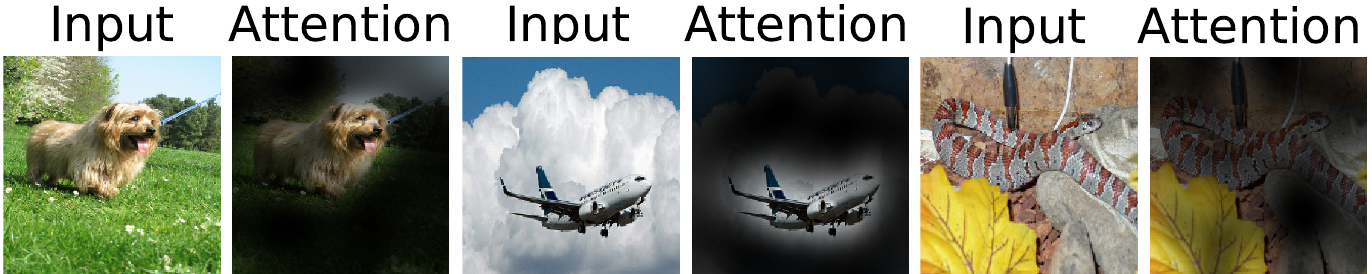
\includegraphics[width=\textwidth]{pictures/vit-attention2}\\
    \caption[Examples of Attention in Vision Transformers]{Representative examples of attention from the output token to the input space of a vision transformer. Figure and caption from~\autocite{Dosovitskiy2021}.}
    \label{fig:vit-attention}
\end{figure}

\begin{figure}[htb]
    \centering
    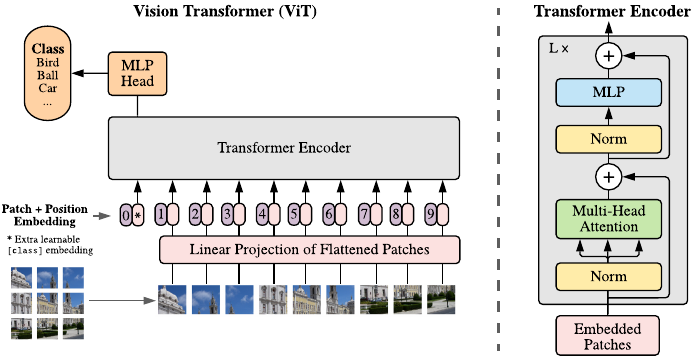
\includegraphics[width=\textwidth]{pictures/vit}\\
    \caption[Vision Transformer Model Structure]{Transformer model overview. An image is split into fixed-size patches, each of them is linearly embedded, the position embeddings are added, and the resulting sequence of vectors fed to a standard transformer encoder. In order to perform classification, an extra learnable ``classification token'' is added to the sequence. Figure and caption from~\autocite{Dosovitskiy2021}.}
    \label{fig:vit}
\end{figure}



% what ViTs can do:
The self-attention mechanism allows the vision transformer to integrate information from across the whole image in all layers, meaning that the receptive field is broad.
This is in contrast to convolutional neural networks, which do tend to have more narrow receptive fields (due to how the convolution algorithm works).
Additionally, transformers are still able to have smaller attention distances in the lower layer, meaning they can resolve local features well, too.
Overall, it was found, that the model attends to image regions that are semantically relevant, as seen in~\autoref{fig:vit-attention}.~\autocite{Dosovitskiy2021}

As mentioned before, for image classification only the classification token is considered, all other features are dropped.
%Transition to unsupervised segmentation
However, as it can be seen in the attention maps, these features contain semantic information about the image, and thus can be used for semantic segmentation~\autocite{Dosovitskiy2021}.
Thus, shortly after the vision transformer was introduced for image classification, algorithms were introduced that utilise these features for image segmentation tasks, for example by adding a projection head, that clusters the features~\autocite{Caron2021}.
It was even found, that features learned in an unsupervised fashion do contain even more relevant information, which can be used for clustering to generate a segmentation map of the input image~\autocite{Caron2021}.

 \subsubsection{Unsupervised Vision Transformer DINO}
% DINO - interpreting feature/attention maps, but make it self-supervised
Features learned in an unsupervised way often provide a richer signal than supervised features, since limiting the training to predefined concepts (for example to classification categories) reduces the rich visual information an image contains~\autocite{Caron2021}.
With unsupervised learning, information of an image assigned to another category might be utilised to build meaningful representations of that category or even other categories or semantic concepts.
%For example, learning representations of sky, even though that was not the intention of detecting street signs, might be helpful to figure out a scene.

In 2021, \citeauthor{Caron2021} set a new state-of-the-art for unsupervised segmentation algorithms with an algorithm called \gls{dino}\footnote{Knowledge distillation is a learning paradigm, where a student network is trained to match a teacher network~\autocite{Caron2021}.}.
It uses a pair of vision transformers as student and teacher networks ($g_{\theta_s}$ and $g_{\theta_t}$) to distill\footnote{Other networks can be used as backbone, but vision transformers were found to perform exceptionally well~\autocite{Caron2021}.} the image features (\autoref{fig:dino-structure})~\autocite{Caron2021}.

\begin{figure}[htb]
    \centering
    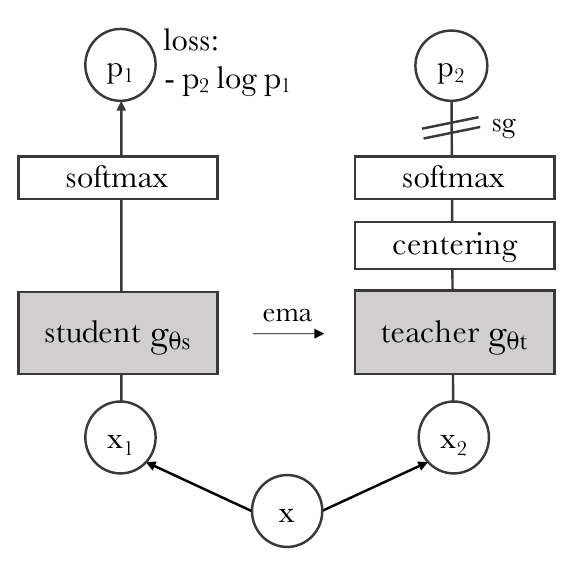
\includegraphics[width=0.55\textwidth]{pictures/dino-structure}\\
    \caption[Structure of DINO]{Self-distillation with no labels. Illustration of DINO in the case of one single pair of views ($x_1$ , $x_2$ ) for simplicity. The model passes two different random transformations of an input image to the student and teacher networks. Both networks have the same architecture but different parameters. The output of the teacher network is centered with a mean computed over the batch. Each network outputs a $k$ dimensional feature that is normalized with a temperature softmax over the feature dimension. Their similarity is then measured with a cross-entropy loss. We apply a stop-gradient (sg) operator on the teacher to propagate gradients only through the student. The teacher parameters are updated with an exponential moving average (ema) of the student parameters. Figure and caption from~\autocite{Caron2021}.}.
    \label{fig:dino-structure}
\end{figure}

The forward pass in each of these two network is calculated as followed, (where $\tau_s > 0$ is a temperature parameter to control sharpness of the output distribution):
\begin{equation}
    P_s(x)^{(i)} = \frac{exp(g_{\theta_s}(x)^{(i)} / \tau_s)}{exp(\sum^K_{k=1}g_{\theta_s}(x)^{(k)} / \tau_s)}
    \label{eq:forward-pass}
\end{equation}

The example given is for the student network, but since student and teacher architecture are the same, output of the teacher will be calculated analogously.

%backwardspass
The loss function of the student network is the cross-entropy loss between teacher and student, while the weight update for the teacher is done by an exponential moving average from the student's weights (also known as momentum encoder)~\autocite{Caron2021}.
For training, each network gets different crops of the same image (taken from a set of views $V$ of the image), but only global crops $x^g_i$ (comprising more than half the input image) are passed to the teacher, while the student gets local and global crops, to encourage a local-to-global correspondence~\autocite{Caron2021}.
Thus, the loss function in the student to be minimised is  (with $H$ being the cross entropy loss $H(a,b) = -a \log(b)$):
\begin{equation}
    \min_{\theta_s} \sum_{x \in \{x^g_1, x^g_2\}} \sum_{\substack{x' \in V \\ x' \neq x}} H(P_t(x), P_s(x'))
    \label{eq:loss-with-crops}
\end{equation}
The weight update in the teacher will be done by an exponential moving average from the student's weights.
Additionally, to avoid collapse in the teacher network, centering and sharpening is used on the output before applying the softmax function.\footnote{There were found two forms of collapse: regardless of the input, the model output is either uniform along all the dimensions or dominated by one dimension.}
Centering was found to hinder one dimension to dominate, but may encourage collapse to a uniform distribution.
Sharpening has an opposite effect.
So, combining both was found to stabilise the model.~\autocite{Caron2021}

% results of DINO
When evaluating this set-up, the authors found that different segmentation heads did attend to different semantic regions of an image even when they were occluded, meaning they were specialised to detect certain semantic patterns~\autocite{Caron2021}.
Additionally, the self-attention maps associated with a classification token\footnote{The name of this now unsupervised token was maintained for consistency with previous works.} showed that the architecture automatically learned class-specific features, as seen in~\autoref{fig:dino-attentionmaps}.
Even though neither the training objective nor the architecture were designed for such dense tasks, the self-attention maps of the vision transformer could be used straight away as segmentation maps, as seen in~\autoref{fig:dino-attentionmaps}~\autocite{Caron2021}.
This underlines the huge potential the self-attention maps of an unsupervised Vision Transformer have.

Not long after \gls{dino} was published, an architecture followed which expanded \gls{dino} by adding an energy-based graph optimisation to better generate segmentation masks from the self-attention maps~\autocite{Hamilton2022}.
This architecture is called \glsfirst{stego}.

\begin{figure}[htb]
    \centering
    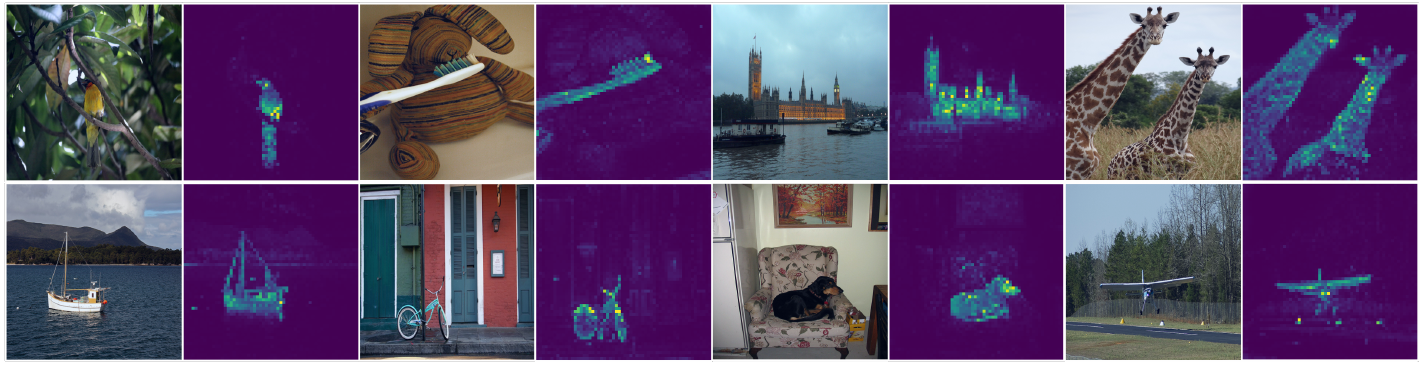
\includegraphics[width=\textwidth]{pictures/dino-attentionmaps}\\
    \caption[Self-attention Maps of DINO]{Self-attention from a vision transformer with 8 × 8 patches trained with no supervision. We look at the self-attention of the classification token on the heads of the last layer. This token is not attached to any label nor supervision. These maps show that the model automatically learns class-specific features leading to unsupervised object segmentations. Figure and caption from~\autocite{Caron2021}.}
    \label{fig:dino-attentionmaps}
\end{figure}
